%!TEX TS-program = xelatex
\documentclass[]{friggeri-cv}
\usepackage{afterpage}
\usepackage{hyperref}
\usepackage{color}
\usepackage{xcolor}
\usepackage{smartdiagram}
\usepackage{fontspec}
% if you want to add fontawesome package
% you need to compile the tex file with LuaLaTeX
% References:
%   http://texdoc.net/texmf-dist/doc/latex/fontawesome/fontawesome.pdf
%   https://www.ctan.org/tex-archive/fonts/fontawesome?lang=en
%\usepackage{fontawesome}
\usepackage{metalogo}
\usepackage{dtklogos}
\usepackage[utf8]{inputenc}
\usepackage{tikz}
\usetikzlibrary{mindmap,shadows}
\hypersetup{
    pdftitle={},
    pdfauthor={},
    pdfsubject={},
    pdfkeywords={},
    colorlinks=false,           % no lik border color
    allbordercolors=white       % white border color for all
}
\smartdiagramset{
    bubble center node font = \footnotesize,
    bubble node font = \footnotesize,
    % specifies the minimum size of the bubble center node
    bubble center node size = 0.5cm,
    %  specifies the minimum size of the bubbles
    bubble node size = 0.5cm,
    % specifies which is the distance among the bubble center node and the other bubbles
    distance center/other bubbles = 0.3cm,
    % sets the distance from the text to the border of the bubble center node
    distance text center bubble = 0.5cm,
    % set center bubble color
    bubble center node color = pblue,
    % define the list of colors usable in the diagram
    set color list = {lightgray, materialcyan, orange, green, materialorange, materialteal, materialamber, materialindigo, materialgreen, materiallime},
    % sets the opacity at which the bubbles are shown
    bubble fill opacity = 0.6,
    % sets the opacity at which the bubble text is shown
    bubble text opacity = 0.5,
}

\addbibresource{bibliography.bib}
\RequirePackage{xcolor}
\definecolor{pblue}{HTML}{0395DE}

\begin{document}
\header{Wesley}{ Banfield}
      {\hspace{5.05cm}Unconventional Thinker - Geologist - Software Engineer}
      
% Fake text to add separator      
\fcolorbox{white}{gray}{\parbox{\dimexpr\textwidth-2\fboxsep-2\fboxrule}{%
.....
}}

% In the aside, each new line forces a line break
\begin{aside}
  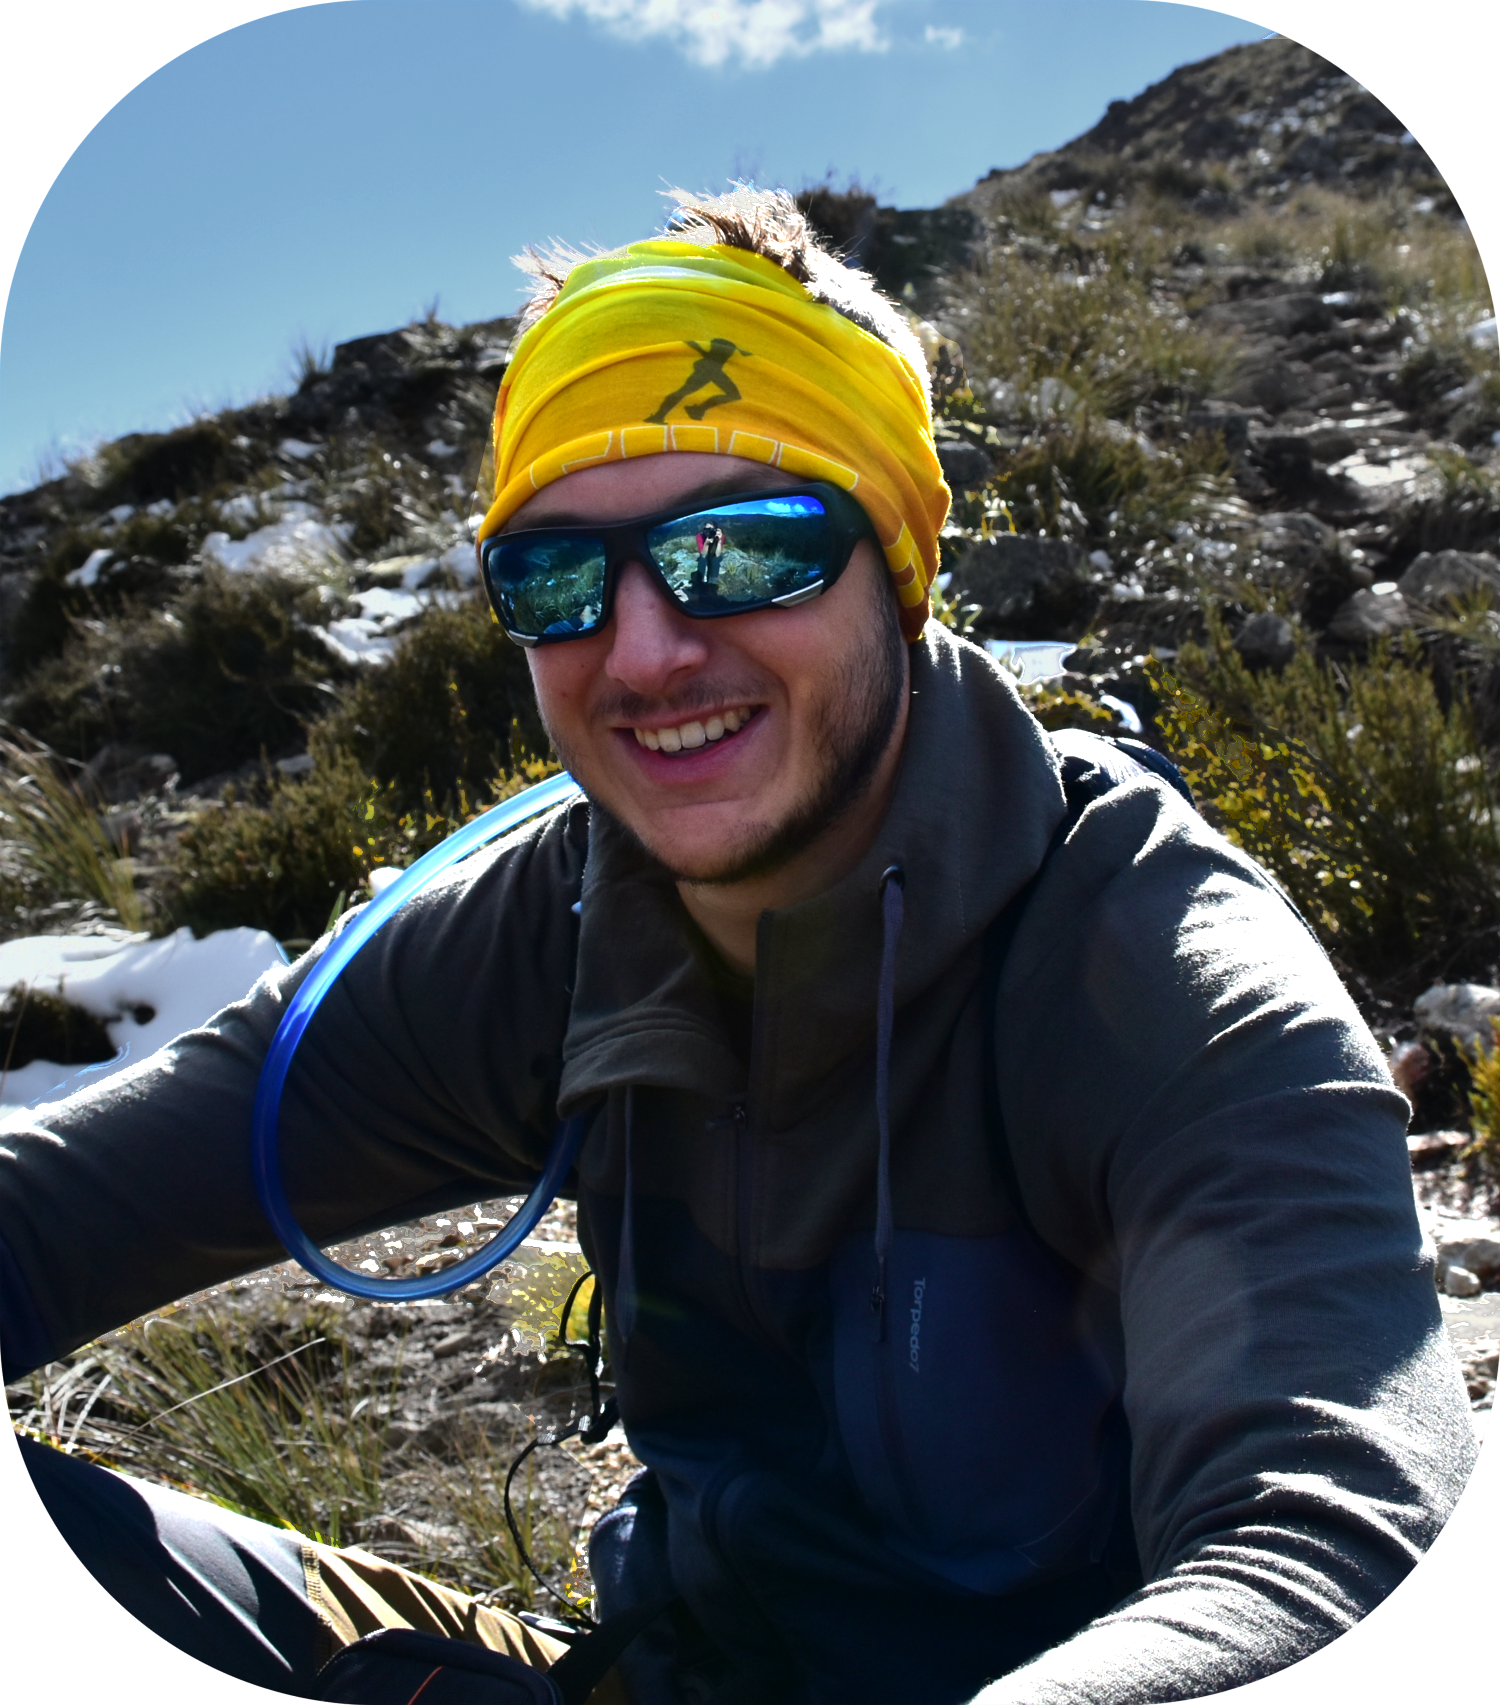
\includegraphics[width=3.5cm]{img/profile_relaxed.png}
  
\includegraphics[width=3.5cm]{img/QR.png}
  \section{Contact}
    \href{mailto:wesleybanfield@gmail.com}{\textbf{wesleybanfield@}\\gmail.com}\vspace{3pt}
    +64 27 777 55 09\vspace{3pt}
    25A Beckford Road,
    Christchurch, 8022
  \section{Web \& Git}
    \href{https://www.linkedin.com/in/wesleybanfield/}{Linkedin}
    \href{https://github.com/WesleyTheGeolien}{Github}
  % use  \hspace{} or \vspace{} to change bubble size, if needed
  \section{Technologies}
	\textbf{Jupyter}
\includegraphics[scale=0.40]{img/4stars.png}
	\textbf{Orange}
\includegraphics[scale=0.40]{img/4stars.png}
	\textbf{Plotly/Dash}
\includegraphics[scale=0.40]{img/4stars.png}
	\textbf{Sklearn}
\includegraphics[scale=0.40]{img/3stars.png}
	\textbf{Docker}
\includegraphics[scale=0.40]{img/3stars.png}
	\textbf{Microsoft PowerApps / Flow}
\includegraphics[scale=0.40]{img/2stars.png}
	~
  \section{Languages}
	\textbf{Python}
\includegraphics[scale=0.40]{img/5stars.png}
	\textbf{C++}
\includegraphics[scale=0.4]{img/3stars.png}
	\textbf{\LaTeX}
\includegraphics[scale=0.4]{img/4stars.png}
	~ 
	~
  \section{Geological Software}
	\textbf{LeapFrog}
\includegraphics[scale=0.40]{img/5stars.png}
	\href{http://www.ccgalberta.com/}{\textbf{CCG}}
\includegraphics[scale=0.40]{img/5stars.png}
	\href{http://www.pdgm.com/products/skua-gocad/}{\textbf{Skua}}
\includegraphics[scale=0.40]{img/3stars.png}
	\textbf{QGis}
\includegraphics[scale=0.40]{img/3stars.png}
	\href{https://snowdengroup.com/software/supervisor/}{\textbf{Supervisor}}
\includegraphics[scale=0.40]{img/3stars.png}
	~
%  \section{Personal Skills}
%    \smartdiagram[bubble diagram]{
%        \textbf{Team}\\\textbf{Player},
%        \textbf{Initiative},
%        \textbf{Curiosity},
%        \textbf{Problem}\\\textbf{Solving},
%        \textbf{\vspace{2mm}Manage\vspace{2mm}},
%        \textbf{Organize}
%    }
    ~
\end{aside}
~
\begin{quote}
\large	
Disruption occurs when you are not paying attention and staying at the forefront of innovation is key. Oil \& Gas Geologist by trade with specialisation in Software Engineering I strive to \textbf{unite technology and innovation} to push the boundaries of what’s possible.
\end{quote}
\section{Experience}
\begin{entrylist}
  \entry
    {01/17 - Now}
    {Research Engineer}
    {\href{https://www.seequent.com/}{Seequent, Christchurch New Zealand}}
    {I pride myself with thinking laterally and outside the box to provide novel innovative solutions, drawing on insights from both my geological and software engineering background.
    
    This role permitted vast exposure to the company and it's clients. Regular client meetings and presentations were held as well as working, and leading, interdisciplinary innitiatives.
    \\[6pt]
   	\textbf{New Technologies} Some problems call for thinking outside the box and implementing new technologies from the base up. Some of these projects included web based dashboard creation, integration of Jupyter and cloud computing.
   	\\[6pt]
   	\textbf{New Solutions} Other projects include the reuse of core IP in novel manners. For example the automated creation of geological models from sub sets of data to sample geological uncertainty. Presentation of work at Seequent's \href{https://lyceum-perth.seequent.com/}{Perth Lyceum}.
    \\[6pt]
   	\textbf{Core Strategy} Providing technical support for key business decisions including full verification of Geostatistical implementation through construction of an automated test suite and implementation of infrastructure to obtain and analyse usage metrics of Leapfrog software suite. 
    \\
    Reference : \href{mailto:tim.schurr@seequent.com}{Tim Schurr, Solutions Architect}
	}
  \entry
    {05/16 - 19/16}
    {Software Integration Engineering Internship}
    {\href{https://www.total.com/en}{Total, Pau France}}
    {Grids play an important part in coupled Oil \& Gas basin modeling. Too fine, the computation time prevails, too coarse, the calcualtions do not converge. As a software integration engineer I implemented an interface with \href{http://www.ring-team.org/software/ringmesh}{RINGMesh} library to dynamically re-meshing during the simulation.\\ Reference : \href{mailto:tristan.cornu@total.com}{Tristan Cornu, Pore pressure and Rock Mechanics Specialist}}
    \entry
    {02/16 - 05/16}
    {Research Intern}
    {\href{http://www.ring-team.org/}{Ring Research Lab, Nancy France }}
    {Research and implementation of different automatic simultaneous well log correlation algorithms and creation of a SKUA-Gocad plug-in. The work was carried out in the lab that orginally developed SKUA-Gocad before commercialisation by Paradigm. The work was presented and published in the 2016 Ring Meeting. \\Reference : \href{mailto:Guillaume.Caumon@ensg.univ-lorraine.fr}{Guillaume Caumon, Head of Research team}}
    \entry
    {06/15 - 09/15}
    {Software Engineering Internship}
    {\href{https://www.seequent.com/}{Seequent, Christchurch New Zealand}}
    {Design and development of a graphical user interface for geostatistical analysis in Leapfrog 3D Geological modelling suite, later integrated into Leapfrog EDGE. Implementation of different geostatistical algorithms.
    \\
    Reference : \href{mailto:tim.mclennan@seequent.com}{Tim McLennan}}
\end{entrylist}

\vspace*{\fill}
\begin{entrylist}
	\entry
	{09/14 - 05/15}
	{Lab Research Project}
	{\href{http://georessources.univ-lorraine.fr/}{GeoRessources, Nancy France}}
	{Geochemistry can be used to date Oil, however when in contact with water certain couples reset. The goal of the project was to develop an experimental protocol to analyse the behaviour of the Rhenium / Osmium couple. Automated graphing tools where developed to analyse the ICP-MS results.
		\\
		Reference : Raymond Michels}
\end{entrylist}
\section{Education MEng, MSc}
\begin{entrylist}
  \entry
    {2013 - 2016}
    {Masters in Geological Engineering with specialisation in Numerical Geology and Oil \& Gas Engineering}
    {\href{http://ensg.univ-lorraine.fr/english/}{French National School of Geological Engineering}}
    {Ecole National Superieur de Geologie is a leading French engineering school specialising in geosciences and delivering a 5 year University Diploma. An extra Masters was at the University of Lorraine was also obtained.\\ \emph{Curriculum}: Oil and Gas Engineering and Numerical Geology\\ 
    \emph{Main subjects}: Structural Geology, Petroleum Systems, Sedimentology, Geomechanics, Mathematical concepts of geomodelling, Software Development, Interface Design, Computer Geometry, Visualisation and Parallelism, Finite Elements.\\
    \emph{Title of Thesis}: ”Current automatic well log correlation techniques, their advantages and drawbacks”.
    \emph{Relators}: Prof. Guillaume Caumon, Jonathan Edwards\\}
  \entry
    {2011 - 2013}
    {\href{https://en.wikipedia.org/wiki/Classe_preparatoire_aux_grandes_ecoles}{Classes Preparatoire aux Grandes Ecoles}}
    {Lycee Pierre de Fermat, Toulouse France}
    {2 years of intensive general scientific courses before national exams for entry to the French Grandes Ecoles, carried out at Pierre de Fermat, one of the top prep classes, 6 / 52\\ 
    \emph{Main subjects}: Geology, Mathematics, Physics, Chemistry and Biology.\\}
\end{entrylist}
\vspace*{\fill}

\end{document}
